\documentclass{standalone}
\usepackage{tikz}
\usetikzlibrary{arrows.meta}
\tikzset{label/.style = {inner sep=1pt, fill=white}}
%\tikzset{nd/.style={circle, inner sep=0pt}}
\tikzset{nd/.style={inner sep=1pt}}
\tikzset{>=Latex}
\tikzset{arc/.style = {->, semithick, >=Latex}}
\begin{document}
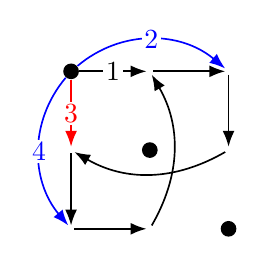
\begin{tikzpicture}

    \node[nd] (1) at (0,0) {};
    \node[nd] (2) at (1,0) {};
    \node[nd,fill, circle,inner sep=2pt] (3) at (2,0) {};
    \node[nd] (4) at (0,1) {};
    \node[nd,fill,circle,inner sep=2pt] (5) at (1,1) {};
    \node[nd] (6) at (2,1) {};
    \node[nd,fill,circle,inner sep=2pt] (7) at (0,2) {};
    \node[nd] (8) at (1,2) {};
    \node[nd] (9) at (2,2) {};
    
    \draw[arc] (4) to (1);
    %\draw[arc] (3) to[in = -40, out = 220] (1);
    %\draw[arc] (3) to[out = 50, in = -50] (9);
    \draw[arc] (8) to (9);
    %\draw[arc] (5) to (8);
    %\draw[arc] (5) to (4);
    
    \draw[arc,red] (7) to node[label=above] {3} (4);
    \draw[arc, blue] (7) to[in = 130, out = -130] node[label=above] {4} (1);
    \draw[arc] (7) to node[label=above] {1} (8);
    \draw[arc, blue] (7) to[in = 140, out = 40] node[label=above] {2} (9);
    
    \draw[arc] (1) to (2);
    %\draw[arc] (3) to (2);
    %\draw[arc] (5) to (2);
    \draw[arc] (2) to[in = -60, out = 60] (8);
    %\draw[arc] (3) to (6);
    \draw[arc] (9) to (6);
    %\draw[arc] (5) to (6);
    \draw[arc] (6) to[out = 210, in = -30] (4);

 \end{tikzpicture}
\end{document}